\documentclass{standalone}
\usepackage{tikz}
\begin{document}
	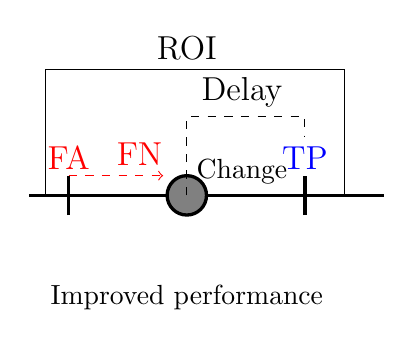
\begin{tikzpicture}[scale=1.0, xscale=1,yscale=1]
		\def\rad{0.25}
		\def\halfh{0.25}
		\draw[black, very thick] (0.5,0) -- (5,0);

		% CHP
		\draw[fill=gray, very thick] (2.5, 0) circle (\rad);
		\node at (3.2, 0.3) {Change};

		% CDE1
		\draw[black, very thick] (1,-\halfh) -- (1, \halfh);
		%\node[below] at (1, -0.3) {\large CDE};
		\node[above, red] at (1, 0.2) {\large FA};

		% CDE2
		\draw[black, very thick] (4,-\halfh) -- (4, \halfh);
		%\node[below] at (4, -0.3) {\large CDE};
		\node[above, blue] at (4, 0.2) {\large TP};
		\node[above] at (3.2, 1.0) {\large Delay};

		% DELAY ARCH
		\draw[dashed] (2.5,0) -- (2.5,1.0) -- (4,1) -- (4, 0.75);

		% FN arrow
		\draw[dashed, red, ->] (1,0.25) -- (2.2,0.25);
		\node[above, red] at (1.9, 0.25) {\large FN};

		\node at (2.5,-1.3) {Improved performance};
        
        % ROI
		\def\hroi{1.6}
		\draw[black] (0.7,0) -- (0.7,\hroi) -- (4.5, \hroi) -- (4.5, 0);
		\node[above] at (2.5, \hroi) {\large ROI};
		
		%%% FOR ALIGNING IN MINIPAGE
		% ROI
		%\def\hroi{1.5}
		%\draw[white] (1,0) -- (1,\hroi) -- (4.5, \hroi) -- (4.5, 0);
		% ARCH
		%\draw[dashed, white] (5,0) to [out=180+70,in=360-70] (2.5,0);
	\end{tikzpicture}
\end{document}
